\chapter{Classificação utilizando aprendizado profundo} \label{chap:class-profundo}
O capítulo \ref{chap:tradicional} tratou-se de uma solução baseada em seleção de candidatos, extração de características e posterior classificação, o que caracteriza uma técnica de aprendizado superficial. Nesse capítulo propomos uma solução híbrida, que utiliza a seleção de candidatos idêntica à anterior, porém utiliza técnicas de aprendizado profundo para classificação, de modo que os candidatos são classificados sem pré-processamento. Inicialmente introduz-se as redes MLP e convolucionais, fornecendo as bases teóricas, funções de ativação e processo treinamento.  Questões relativas à implementação também são abordadas.

\section{Perceptron Multicamadas (MLP)}

Segundo \cite{DLbook}, uma rede perceptron multicamadas (MLP) também pode ser chamada de rede profunda sem realimentação (\textit{deep feedforward networks}) ou de rede neural. Essa estrutura consiste na organização de múltiplos nós organizados em camadas, como ilustra a Figura \ref{fig:mlp}. 
 
Convenciona-se $w_{jk}^l$ como o peso da conexão entre o nó $j$ da camada $l$ e o nó $k$ da camada $(l-1)$, como ilustrado na Figura \ref{fig:bp}. De maneira semelhante, $b^l_j$ e $a^l_j$ indicam o \textit{bias} e a ativação (saída) do nó $j$ da camada $l$ dados por
\begin{equation}
a^l_j = \phi (z^l_j) =\phi \left( \sum_k w_{jk}^l a_k^{l-1} + b_j^l \right)
\end{equation}
onde $\phi(z)$ é a função de ativação da rede. Denota-se por $\theta$ o vetor de parâmetros da rede, composto por todos os parâmetros de pesos $w$ e de \textit{bias} $b$ da rede.

\begin{figure}
\centering
\begin{subfigure}{.5\textwidth}
  \centering
  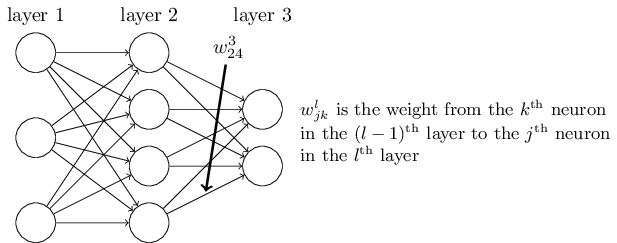
\includegraphics[width=\linewidth]{deep/bp-weights}
\end{subfigure}%
\begin{subfigure}{.5\textwidth}
  \centering
  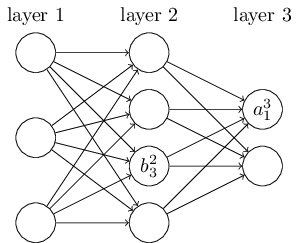
\includegraphics[width=0.8\linewidth]{deep/bp-bias}
\end{subfigure}
\caption{Conveção das conexões entre unidades.}
\label{fig:bp}
\end{figure}

Para o problema de classificação, pode-se utilizar uma rede neural de $L$ camadas: a camada de entrada recebendo a amostra $x$ sem pré-processamento, camadas intermediárias responsáveis pela descrição da amostra e a camada final, que no caso de classificação binária possui uma única unidade, cuja saída $a^L_0$ é a probabilidade da amostra ser positiva. Pode-se denotar, poranto, a saída da rede como a função
\begin{equation}
f(x, \theta) = a^L_0(x, \theta).
\end{equation}

Os hiper-parâmetros da rede consistem no número de camadas, e nos de unidades em cada camada que se deseja utilizar. Para problemas complexos, incluindo imagens de alta resolução com múltiplas classes de objetos pode-se ter mais de vinte camadas intermediárias. Entretanto, para o presente problema, por se tratar de amostras de baixa resolução e reduzida complexidade, utilizam-se apenas duas camadas intermediárias. Além desses, inclue-se nos hiper-parâmetros a função de ativação $\phi(z)$ que se escolhe para cada camada da rede.

\section{Função de ativação}
\label{sec:funcao-ativacao}
Uma função de ativação $\phi(z)$ é responsável por introduzir não-linearidades na rede, um requisito fundamental para ter bom resultado com conjuntos de dados mais complexos. A escolha dessa função está associada à diversos fatores. Um deles é desempenho da rede, especialmente durante treinamento. Outro fator é a interpretação que se dá à saída de uma unidade. Duas funções, escolhidas segundo um desses objetivos, são utilizadas nesse trabalho e são introduzidas a seguir.

\subsection{Sigmoide}
Para classificadores interpreta-se o valor das unidades da camada de saída como probabilidades da amostra pertencer a uma determinada classe. A escolha da função de ativação, nesse caso, se dá justamente pela interpretação da camada de saída. Nesse caso espera-se que os valores estejam no intervalo $[0,1]$. Uma função que assegura essa condição é a sigmoide, ilustrada na Figura \ref{fig:sigmoid}
\begin{equation}
	\label{eq:sigm}
	\sigma(z) = \frac{1}{1+e^{-z}}.
\end{equation}

\begin{figure}
\centering
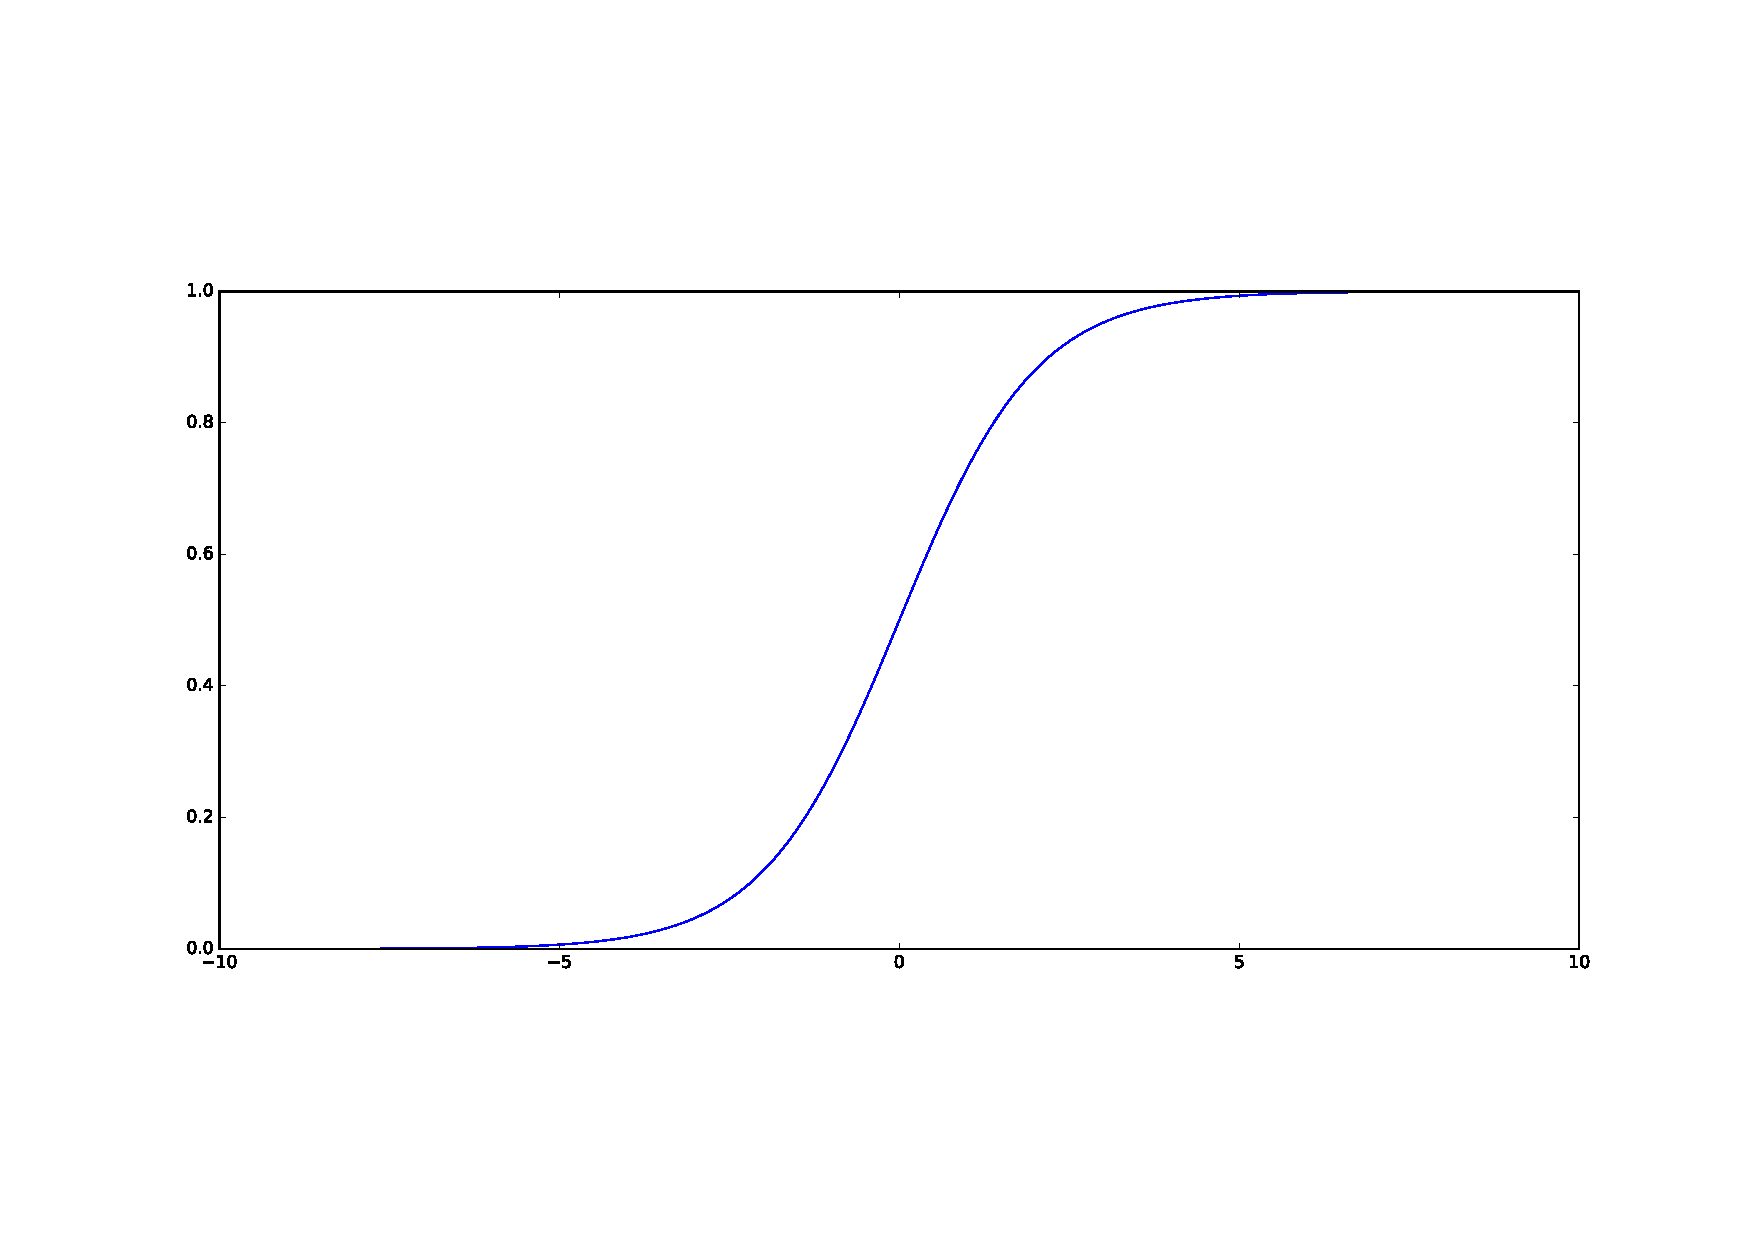
\includegraphics[width=0.5\textwidth]{deep/sigmoid}
\caption{Gráfico mostrando o comportamento da sigmoide.}
\label{fig:sigmoid}
\end{figure}

Historicamente essa função foi utilizada para as camadas intermediárias. No entanto, observa-se que essa função satura facilmente com entradas pŕoximas de 1 ou 0, ocasionando uma derivada praticamente nula nessas regiões. Como destacado na subseção \ref{sub-sec:backprop}, isso é um problema ao se considerar que a derivada dessa função definirá a atualização dos pesos desses nós durante o processo de treinamento. Ao propagar esse processo camada a camada, verificam-se derivadas cada vez menores, o que causa o problema do gradiente enfraquecido, em que as camadas iniciais não conseguem aprender pois o gradiente é muito reduzido.

\subsection{RELU}
Para resolver o problema do gradiente enfraquecido, obtendo uma melhora no desemepenho da rede, a função RELU (\textit{Rectified Linear Unit}), ilustrada na Figura \ref{fig:relu}, foi proposta \cite{nair2010relu} como
\begin{equation}
	\label{eq:relu}
	\text{RELU}(z) = \max\{0,z\}.
\end{equation}

\begin{figure}
\centering
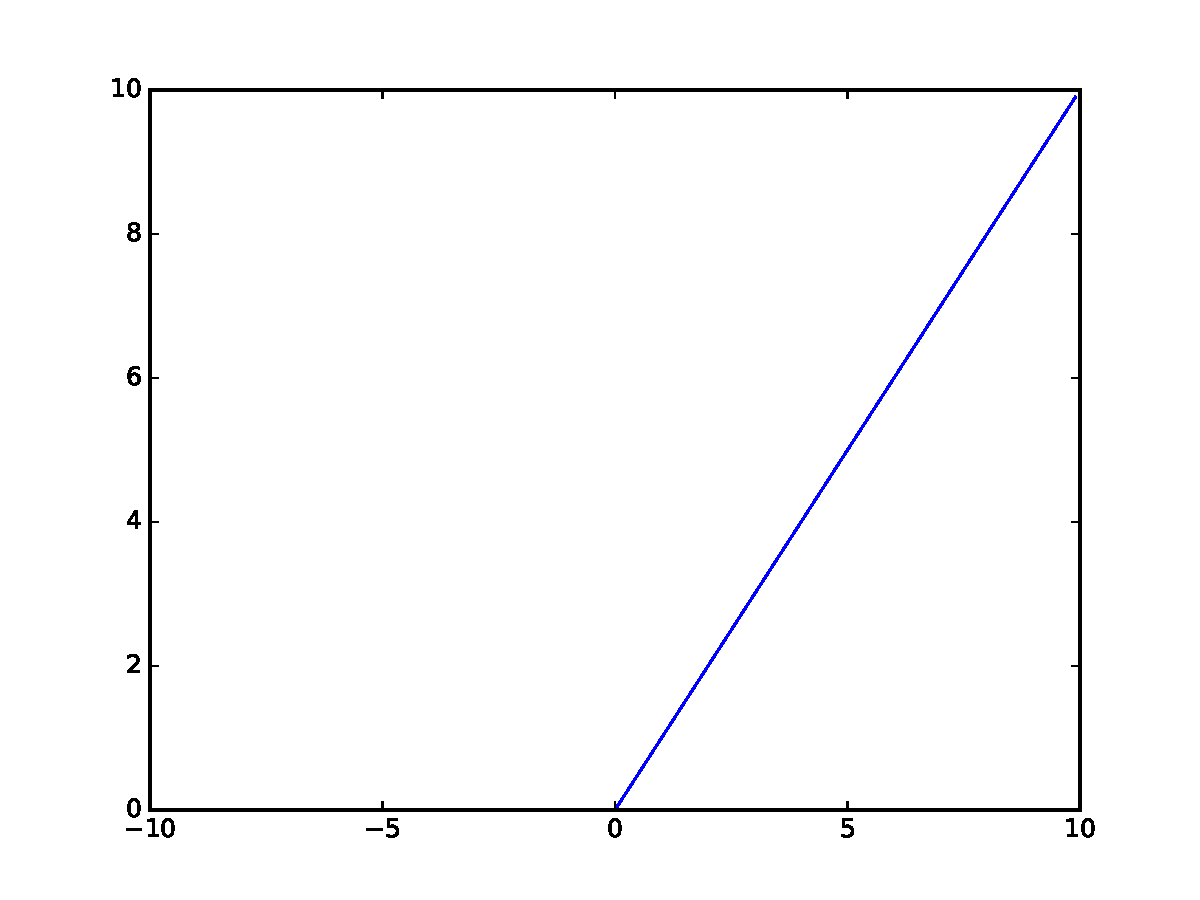
\includegraphics[width=0.5\textwidth]{deep/relu}
\caption{Gráfico mostrando o comportamento da função RELU.}
\label{fig:relu}
\end{figure}

Observa-se que para valores positivos essa função tem uma derivada constante e igual a um, proporcionando um gradiente considerável sempre que o nó estiver ativo. Por outro lado, para valores negativos considera-se o nó inativo e os pesos não são atualizados. Essas características garantem boa propagação do gradiente, portanto essa função de ativação é usualmente utilizada para as camadas intermediárias da rede, mantendo, ainda, a ativação sigmóide para a camada de saída.

\section{Treinamento}
Uma maneira de avaliar o desempenho de uma rede é através da avaliação da chamada função custo. O processo de treinamento de uma rede neural é justamente o problema de otimização dessa função. Porém, diferentemente do caso do SVM, trata-se de uma otimização não convexa, isto é, existem múltiplos mínimos locais para essa função e diversas soluções podem ser encontradas, dependendo dos valores iniciais dos parâmetros. Esse fato advém do caráter não linear das funções de ativação nas diferentes camadas da rede.

Durante essa etapa otimiza-se os parâmetros $\theta$ de forma que $y_i \approx f(x_i, \theta)$ para o conjunto de treinamento $\{ (x_i, y_i) | i=1,\dots,N \}$. Isso é feito através da minimização de uma função custo $C(\theta)$ por um algoritmo de otimização chamado SGD (\textit{Stocastic Gradient Descent}) utilizando o gradiente de $C$ obtido por um algoritmo de propagação reversa de erros. Todos esses passos são descritos a seguir.

\subsection{Função custo}
A função custo quantifica a qualidade de representação que o modelo oferece para o conjunto de treinamento, isto é, qual a medida de erro que o classificador comete dentro do próprio conjunto de treinamento.

Em geral pode-se escrever a função custo como
\begin{equation}
C(\theta) = \sum_i^N C_i(\theta)
\end{equation}
de forma que se pode calcular o custo de cada amostra de treinamento individualmente, correspondente ao erro equivalente àquela amostra.

Introduz-se a função custo de entropia cruzada binária (\textit{binary cross entropy}), utilizada no presente trabalho e descrita por
\begin{equation}
\label{eq:bcr}
C(\theta) = -\frac{1}{N} \sum_i^N \left[y_i \ln f(x_i,\theta) + (1-y_i) \ln (1-f(x_i,\theta))\right]
\end{equation}
cuja grande contribuição é permitir o uso de unidades sigmoidais na camada de saída sem enfraquecer o gradiente, visto que a função exponencial da ativação é revertida ao se utilizar o logaritmo natural imposto pela entropia cruzada. Nota-se ainda, no caso em que $f(x,\theta)=y \in \{0, 1\}$ tem-se um custo nulo dessa função.

É interessante notar, ainda, como essa função penaliza amostras cuja saída da rede $f(x_i,\theta)$ difere do valor especificado no treinamento $y_i$ conforme ilustra a Figura \ref{fig:plot-cost}.

\begin{figure}
\centering
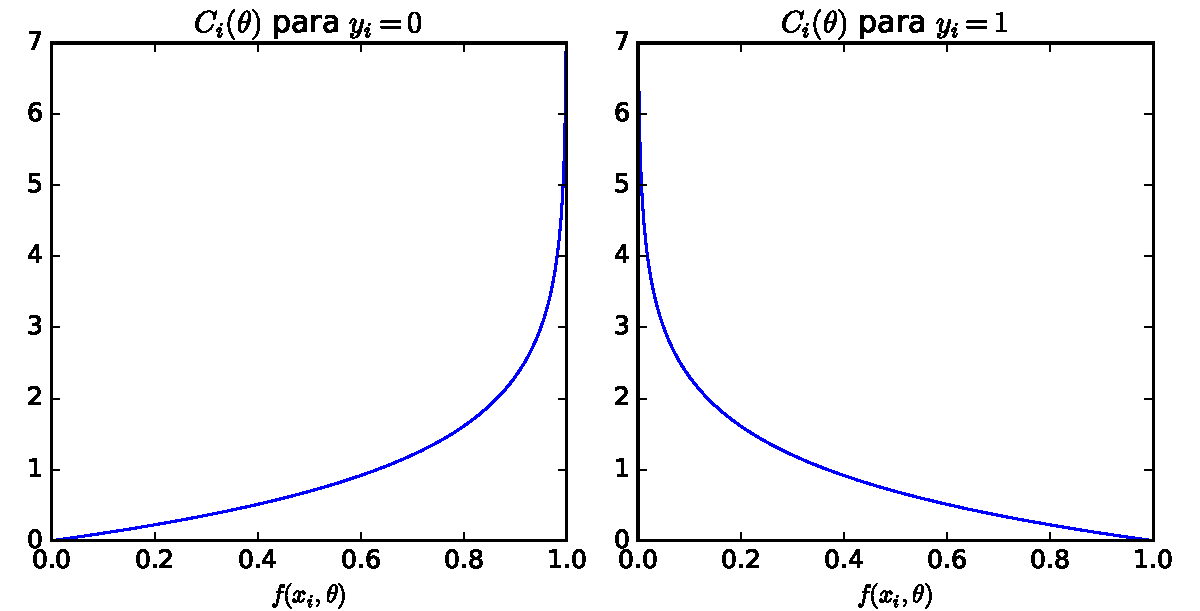
\includegraphics[width=0.8\textwidth]{deep/cross-entropy-loss}
\caption{Comportamento da função custo entropia cruzada para amostras negativas (esquerda) e positivas (direita).}
\label{fig:plot-cost}
\end{figure}

Tendo uma métrica para avaliar a qualidade do classificador em relação ao conjunto de treinamento utiliza-se um algoritmo de otimização para encontrar parâmetros que melhoram o desempenho desse mecanismo.

\subsection{\textit{Stochastic Gradient Descent}}
\label{sec:sgd}
Um método tradicional para minimização é o do gradiente descendente, que utiliza a aproximação
\begin{equation}
\Delta C \approx \nabla C \cdot \Delta \theta
\end{equation}
para verificar a variação $\Delta C$ na função custo em função do gradiente $\nabla C$ e na variação nos parâmetros $\theta$. Basicamente escolhe-se os parâmetros inicialmente aleatórios e então busca-se encontrar o vetor de variação dos parâmetros $\Delta \theta$ que façam C diminuir. Ao escolher $\Delta \theta = -\eta \nabla C$, tem-se
\begin{equation}
\Delta C = -\eta \abs{\nabla C}^2
\end{equation}
que será negativo ao escolher $\eta > 0$, chamada de taxa de aprendizado (\textit{learning rate}). Esse processo é executado iterativamente, atualizando os parâmetros com $\theta \gets \theta + \Delta \theta$ até se encontrar um mínimo local.

Em geral redes profundas necessitam de um grande número de amostras para serem treinadas. O cálculo do gradiente $\nabla C$ é custoso ao se considerar a quantidade amostras, visto que $\nabla C = \sum_i^N \nabla C_i$. Utiliza-se, então, uma variação do método chamada de \textit{Stochastic Gradient Descent} -- SGD. Essa variação particiona o conjunto de treinamento aleatóriamente em $M$ subconjuntos, chamados \textit{mini batches}. Os índices das amostras do $m$-ésimo \text{mini batch} compôem o conjunto de índices $I_m$, de maneira que $I_1, I_2,\dots \subseteq \{1,\dots,N\}$. Então estima-se o gradiente total fazendo a soma dos gradientes individuais como
\begin{equation}
\nabla C \approx \sum_{i \in I_m} \nabla C_i
\end{equation}
ou seja, avaliando o gradiente gradiente apenas nas amostras percentences ao $m$-ésimo \textit{mini batch} a cada iteração do método, o que reduz drasticamente o tempo de execução do algoritmo.

Nota-se ainda que a nomenclatura \textit{Stochastic Gradient Descent} se refere ao caso particular quando $M=1$, porém será utilizada nesse trabalho mesmo para valores de $M$ maiores que um.

\subsection{Backpropagation}
\label{sub-sec:backprop}
%neuralnetworksanddeeplearning.com/chap2.html

O método de otimização visto na seção \ref{sec:sgd} faz uso do gradiente de função custo $\nabla C$, porém não mostra como calcular essa quantidade. Para isso é necessário encontrar as derivadas da função custo em relação aos parâmetros individuais de cada elemento da rede, $w$ e $b$. De fato, utilizar as ferramentas do cálculo se mostra um desafio na prática, visto a complexidade da função custo em termos da função da rede $f(x, \theta)$ que combina todas as não linearidades encadeadas nas camadas. 

Uma solução foi o algoritmo de propagação reversa de erros (\textit{backpropagation}), já existente na década de 1979 porém proposto mais recentemente em \cite{backpropagation}, que fornece um método eficiente de calcular as derivadas da função custo em relação a quaisquer parâmetros $w$ e $b$ da rede.

Primeiramente define-se uma grandeza intermediária chamada de erro da camada $l$, $\delta^l$, interpretada como a contribuição da camada $l$ para o erro total, através do qual serão calculadas as grandezas de interesse.

Esse algoritmo possui uma formulação complexa que não está no escopo desse trabalho. Entretanto, alguns aspectos serão enfatizados pela análise simples das equações fornecidas por esse método, disponíveis com demonstração em \cite{NeuralNetsDeep}, vistas a seguir:
\begin{align}
\delta^L &= (a^L - y) \odot \phi^\prime(z^L) \label{eq:deltaL} \\ 
\delta^l &= ((w^{l+1})^T\delta^{l+1}) \odot \phi^\prime(z^l) \label{eq:deltal}\\
\pd{C}{b_j^l{}} &= \delta_j^l \label{eq:delCb}\\ 
\pd{C}{w_{jk}^l{}} &= a_k^{l-1} \delta_j^l \label{eq:delCw}
\end{align}
onde $\odot$ é o operador de multiplicação elemento por elemento.

Pode-se entender o algoritmo como calculando o erro na camada de saída, $\delta^L$ com \eqref{eq:deltaL} (simplificada para um caso específico função custo) e propagando esse erro para as outras camadas, com a contribuição individual de cada unidade, obtendo os correspondentes $\delta^l$ conforme \eqref{eq:deltal}. Através dos quais as demais derivadas são obtidas, através de \eqref{eq:delCb} e \eqref{eq:delCw}, e permitem obter o gradiente da função custo. 

Um aspecto a destacar é o papel fundamental da derivada da função de ativação $\phi(z)$ em \eqref{eq:deltal}. Se ela saturar, essa derivada terá um valor baixo, o que provoca um gradiente pequeno e a atualização dos parâmetros fica estagnada, impedindo o aprendizado. Por isso a importância de funções de ativação que impedem a saturação, como a RELU, vista anteriormente.

Nota-se ainda que a equação \eqref{eq:delCw} mostra que a derivada da função custo em relação ao pesos de um determinado nó é proporcional à entrada correspondente ao nó de entrada. Portanto, caso a entrada seja nula, essa componente do gradiente será também nula, o que significa que o nó só tem seu peso atualizado quando estiver ativo.

\section{Redes convolucionais}
\label{sec:convnets}
%http://neuralnetworksanddeeplearning.com/chap6.html#introducing_convolutional_networks

A estrutura MLP vista anteriormente é chamada de completamente conectada, onde cada unidade em uma camada está conectado à todas as demais da próxima camada. Uma variante desse modelo são as chamadas redes convolucionais, que introduzem um aspecto espacial no processamento das amostras de forma que as camadas possuam uma estrutura. São especialmente úteis para amostras de maior dimensão que têm uma estrutura matricial, como imagens. Se destacam em relação à MLP pois a relação de estrutura não precisa ser incorporada ao modelo via treinamento mas já advém diretamente do modelo utilizado.

Apesar de já existirem na década de 1970 considera-se que o trabalho \cite{lecun1998convnet} foi fundamental para estabelecer a teoria moderna das redes convolucionais. Essas redes continuam organizadas em camadas, porém não são completamente conectadas. Conectam-se as camadas através dos chamados campos receptivos locais (\textit{local receptive fields}) que ligam uma série de nós da camada anterior à próxima, como ilustra a figura \ref{fig:convnet-receptivefield}. Os campos receptivos são transladados para obter as conexões dos próximos nós na camada intermediária.

\begin{figure}
\centering
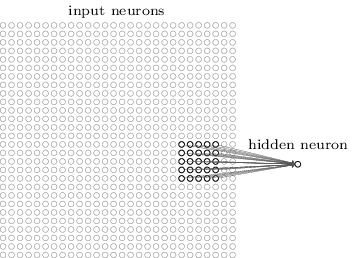
\includegraphics[width=0.5\textwidth]{deep/convnet-receptivefield}
\caption{Exemplo de rede convolucional e campos receptivos.}
\label{fig:convnet-receptivefield}
\end{figure}

Além desse aspecto de estrutura introduzido pelos campos receptivos, tem-se que os pesos e \textit{bias} são compartilhados pelos diferentes campos receptivos. Isto é, para cada nó da camada intermediária embora as ligações ocorram com diferentes nós da camda anterior, elas compartilham o mesmo peso e isso reduz drasticamente a quantidade de parâmetros da rede, tornando o processo de treinamento mais rápido. Portanto tem-se que os diferentes campos receptivos são sensíveis à um mesmo padrão ou característica (\textit{feature}) e isso garante uma invariância à translação. Os pesos compartilhados são também chamados de núcleo (\textit{kernel}). De fato, observa-se que essa operação é resumida como uma convolução entre a camada anterior e o núcleo:
\begin{equation}
a^1 = \phi(w \ast a^0 + b) 
\end{equation}
onde $a^0$ é a camada anterior e $a^1$ o primeiro mapa de características, sendo $\phi(z)$ a função de ativação e $w$ o núcleo.

Na prática, entretanto, utilizam-se múltiplos núcleos de maneira a obter um mapa de características mais rico. Isso significa aumentar drasticamente a dimensionalidade da rede e implica na necessidade de utilizar camadas de \textit{pooling} que reduzam a dimensionalidade da rede através de uma amostragem. Uma das possibilidades é utilizar \textit{max-pooling}, uma técnica de amostragem não linear. Esse método divide o mapa em blocos de tamanhos iguais especificados e para cada bloco seleciona o maior valor, descartando os demais e portanto reduzindo dimensionalidade. Basicamente condensa-se a informação sobre a característica que se deseja encontrar reduzindo o impacto da sua localização exata.

Por fim, após camadas convolucionais e de amostragem, tem-se mapas de características densos, que podem em seguida serem utilizados por uma camada densamente conectada para realizar o processo final de classificação, como ilustrado na Figura \ref{fig:convnet}. 

O processo de treinamento é similar às MLPs, porém com pequenas modificações dado o caráter estrutural e convolucional da rede.

\section{Implementação}
A solução híbrida proposta nesse capítulo assume que os candidatos são obtidos através do algoritmo tradicional visto na seção \ref{sec:tradicional-candidatos} e utiliza um classificador profundo sem que haja pré-processamento das amostras. Dois tipos de estruturas foram utilizadas, primeiramente uma rede MLP e em seguida uma rede convolucional. 

Para ambas as estruturas é necessário especificar qual a topologia da rede: número de camadas e de nós em cada camada, tamanho dos filtros convolutivos e de amostragem, funções de ativação e método de inicialização de pesos e de otimização.  A seleção desses parâmetros pressupõe o entendimento do funcionamento da rede e um ajuste fino baseados em experimentos empíricos pode melhorar o desempenho do classificador.

Existem diversas plataformas para se implementar redes neurais. Entre essas, destacam-se a biblioteca de código aberto \textsc{Theano} \cite{theano}, que permite a definição de e avaliação de expressões matemáticas multidimensionais, diferenciação simbólica, otimização para velocidade e estabilidade, além de uso transparente da GPU. Essa biblioteca, entretanto, não fornece funções específicas para a criação de redes neurais, ou seja, é necessário que o usuário crie as matrizes de pesos, defina função custo e de ativação e implemente o algoritmo de propagação reversa.

Para facilitar a utilização das técnicas de aprendizado profundo e tornar o processo de desenvolvimento mais rápido, utilizou-se a a biblioteca \textsc{Keras} \cite{keras}, que fornece uma abstração acima do \textsc{Theano}. Isso permite criar redes com poucas linhas de código, definindo camadas de maneira simples e escolhendo as funções de ativação e custo dentre as já definidas. Ainda assim, permite flexibilidade para o usuário criar suas próprias funções e ajustar parâmetros da rede, assim como processos de inicialização dos parâmetros e diferentes tipos de otimizadores.

Ambas as bibliotecas são desenvolvidas para \textsc{Python} e portanto houve a necessidade de integrar esse código ao já existente em C++. Destaca-se a dificuldade em integrar o funcionamento paralelo dos algoritmos sob a plataforma CUDA. Isso se deve ao fato do código em C++ referente ao processamento das imagens de profundidade e ao \textsc{Theano} utilizarem simultaneamente os recursos da GPU. Esse conflito foi resolvido utilizando um sistema de troca de contextos proviente da própria plataforma CUDA.

Outro problema enfrentado ocorreu durante a etapa de treinamento. O conjunto de dados utilizado é fortemente desbalanceado, onde mais de 89\% das amostras pertence à classe negativa. Após a primeira etapa de treinamento observou-se uma acurácia de aproximadamente 89\%, o que era aparentemente um ótimo resultado. Entretanto faltou a consideração da distribuição desses resultados: o classificador indicava todas as amostras como sendo negativas, pois o conjunto de dados é altamente enviesado. Para corrigir esse problema listou-se duas opções: equilibrar o conjunto de dados ou modificar a função custo para ponderar os pesos para as classes. Verificou-se que a distribuição de classes pôde ser artificialmente equilibrada replicando as amostras positivas até que seu número se equiparar com as negativas, o que de fato demonstrou um resultado positivo na prática.

Encontrou-se também uma dificuldade para convergência do método utilizando apenas o otimizador SGD. A solução foi utilizar uma variante chamada Adam cuja formulação inclui considerações sobre momento, que consiste em adaptativamente corrigir a taxa de aprendizado $\eta$, o que impacta positivamente sobre a convergência da otimização.

